\chapter{Nodal Analysis}

\section{Basic Idea}
A circuit with $b$ branches has $2b$ unknowns since there are $b$ voltages and $b$ currents. Hence, $2b$ linear independent equations are required to solve the circuit. If the circuit has $n$ nodes and $b$ branches, it has
\begin{itemize}
 \item Kirchoff's current law (KCL) equations
 \item Kirchoff's voltage law (KVL) equations
 \item Characteristic equations (Ohm's Law in a broad sense.)
\end{itemize}  
There are only $n-1$ KCLs since the nth equation is a linear combination of the remaining $n-1$. At the same time, it can be demonstrated that if we can imagine a very high number of
closed paths in the network only $b-n+1$ are able to provide independent KVLs.To prove this statement, let us consider a generic electrical circuit. Let us now substitute the circuit with one oriented graph i.e. with a diagram composed of oriented arcs where each arc represents one of the branches of the original circuit.
With this substitution we can focus simply on the topology disregarding the characteristics of the specific branch. In effect our conclusion regarding the KVL must be valid for every network no matter the branches involved and then it makes sense to focus
only on the connections.

\begin{figure}[ht]
	\centering
	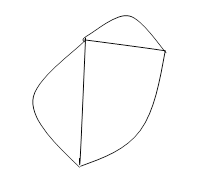
\includegraphics[scale=0.6]{img/graph_representation_1.png} 
	\caption{Graph representing the topology of an electrical circuit}
	\label{fig:graph_rep_1}
\end{figure}

Let us now orient the arc, exactly as we assume to assume a direction for the measurement of the current and let us also number the arcs.

\begin{figure}[ht]
	\centering
	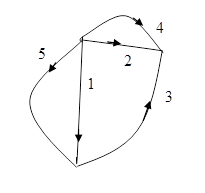
\includegraphics[scale=0.6]{img/graph_representation_2.png} 
	\caption{Oriented graph representing the topology of an electrical circuit}
	\label{fig:graph_rep_2}
\end{figure}

Let us now define a so called tree for this graph. A tree is given by a subset of arcs that connects all the nodes but do not create any closed path.

\begin{figure}[ht]
	\centering
	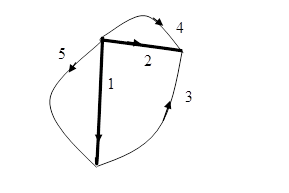
\includegraphics[scale=0.6]{img/graph_representation_3.png} 
	\caption{Selecting a tree of the graph}
	\label{fig:graph_rep_3}
\end{figure}

It is pretty easy to understand that to connect $n$ nodes without creating a closed path we are going to need $n-1$ arcs. As result $b-n+1$ arcs are not included in the tree (this is actually called co-tree).

For this network for example we have:
\begin{align}
\begin{split}
	b &= 5 \\
	n &= 3
\end{split}
\end{align}

So the tree includes 2 branches and the co-tree includes 3 branches.

\section{Resistive Companion Method}

\subsection{Capacitor and Inductor}
These components need some kind of memory since their behavior is dependent on the past.

\begin{equation}
        v_L(t) = L \frac{di_L(t)}{dt} \rightarrow i_L(t) = i_L(t-\delta t)+\frac{1}{L} \int_{t-\delta t}^t v_L(\tau)d\tau
\end{equation}

\begin{equation}
        i_C(t) = L \frac{dv_C(t)}{dt} \rightarrow v_C(t) = v_C(t-\delta t)+\frac{1}{C} \int_{t-\delta t}^t i_C(\tau)d\tau
\end{equation}

